% \documentclass[10pt]{beamer}
\documentclass[10pt,handout]{beamer}

% \usetheme{Pittsburgh}
% \usetheme{metropolis}%great
% \usetheme{hsrm}%BEST for Presentation
% \usetheme{Hannover}%clean white best bright theme
% \usetheme{AnnArbor}%good
% \usetheme{Bergen}
\usetheme{Berkeley}%BEST for Email
% \usetheme{Frankfurt}
% \usetheme{Warsaw}
% \usetheme{sthlm}
% \usetheme{hri}
% \usetheme{Marburg}%amazing


% \usecolortheme{owl} % dark theme
% \usecolortheme[snowy]{owl} % black on white
% \usecolortheme[cautious]{owl}% dark wo redef colors

\usepackage{appendixnumberbeamer}
\usepackage[T1]{fontenc}
\usepackage[utf8]{inputenc}
% \usepackage{lmodern}
% \usepackage{tikz}
\usepackage{textcomp}

\usepackage{booktabs}
\usepackage[scale=2]{ccicons}

% \usepackage{pgfplots}
% \usepgfplotslibrary{dateplot}

\usepackage{xspace}
\usepackage{tabularx}
\renewcommand\tabularxcolumn[1]{m{#1}}% for vertical centering text in X column
\newcolumntype{Y}{>{\centering\arraybackslash}X}
\usepackage{adjustbox}



% \newcommand{\themename}{\textbf{\textsc{metropolis}}\xspace}

\title{ GPUCoin ICO }
\subtitle{Rent excess GPU compute to those in need - Build future proof decentralized video, AI, VR, AR protocols on IPCN™\textsuperscript{TM}
 % or \texttrademark
 - the biggest protocol ICO since File-coin}
\date{\today}
% \author{Hoot AR ads team}
% \institute{Hoot Live inc., a Delaware C-corp}
% \titlegraphic{\hfill
\includegraphics[height=1.5cm]{logo.pdf}}
\author{GPUCoin IPCN
% ™\textsuperscript{TM} 
network protocol team}
\institute{\href{http://gpuco.in}{GPUCoin Foundation}}

\begin{document}
\maketitle

% \begin{frame}{Table of contents}
% \setbeamertemplate{section in toc}[sections numbered]
% \tableofcontents[hideallsubsections]
% \end{frame}

% \section{Primer}
\section{Block-chain decentralization revolution}
\begin{frame}[fragile]{Block-chain decentralization revolution}
	% \begin{itemize}%needs pause
 % \setbeamercovered{transparent}%show dimmed
 % \begin{itemize}[<+->]%uncover piecewise
 \begin{itemize}[<+-| alert@+>]%uncover w highlight 
 
\item Centralized proprietary services are being replaced with \textbf{decentralized open source} services
 % \pause
\item trusted parties replaced with \textbf{verifiable mathematical computation}
% , cryptographic signatures \& public-key cryptography
\item brittle location addresses replaced with \textbf{resilient content addresses}
\item inefficient monolithic services replaced with \textbf{peer-to-peer algorithmic markets}
\item complex inefficient unverifiable data-structures with \textbf{verifiable efficient data-structures, Merkle Trees}
% \item Cryptographic signatures \& public-key cryptography, cryptographic hash functions, cryptographic proof-of-work, time-stamping, Merkle trees, chains of transactions blocks, Byzantine fault tolerance, smart contracts
%FIXME use this line somewhere
\item p2p transfer of value, trust-less computing, non-custodial exchanges, decentralized \textbf{Filecoin} storage, distributed \textbf{GPUCoin} computing - basis for building Ðecentralized applications(Ðapps)

\end{itemize}
 \pause
Ðapps still lack the ability to include streaming media, distributed computing \& data in an open, secure, safe \& decentralized way

\end{frame}
%--- Next Frame ---%

\begin{frame}[t]\frametitle{GPU Mining \& crypto profitability}
 %FIX this slide should show why GPUCoin is the decentralized protocol coin
\begin{itemize}[<+-| alert@+>]
\item GPUs have gotten very powerful thanks to \textbf{Google TPUs} \& \textbf{NVIDIA GPUs} but crypto has not caught on but for \textbf{wasteful HASHCASH mining} \& megatons of CO$_2$ emissions
\item When polymath \textbf{Vitalik Buterin} decides to switch \textbf{ETHereum} to \textbf{Proof-of-stake} system very soon, crytpo miners are going to have excess mining \& null GPU cycles \& capacity
\item Turn these excess data-center \& \textbf{miner NULL GPU/CPU cycles} into valuable crypto-currency GPUCoins(GPCs)
 \item GPUCoin mining is \textbf{profitable} reminiscent of Bitcoin golden days circa 2009-2011
\item GPUCoin will become the main currency for crypto-currency \textbf{Miners} \& save their excess investment when many block-chains become proof-of-stake following ETHereum Vitalik's lead
\end{itemize}
 \pause
 
\includegraphics[scale=0.1]{static/hootcoin} 
\Large{ GPUCoin(GPC) will make crypto-currency mining profitable again in a sustainable manner}

\end{frame}
%--- Next Frame ---%

\begin{frame}[t]{Evolution of Decentralized web \& crypto-currencies}
\textbf{Netscape moment}: \emph{Cambrian} explosion of crypto-currency Ðapps
 
% \newcolumntype{Y}{>{\centering\arraybackslash}X}

 \begin{adjustbox}{width=.75\textwidth}
\begin{tabularx} {\textwidth}{|X|X|X|X|}
 \hline
& 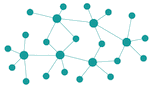
\includegraphics[scale=0.2]{static/decentnew} & 
\includegraphics[scale=0.2]{static/hootcoin} & \\
 \hline
\textbf{Phase} & \textbf{Internet} & \textbf{Crypto-currency} & \textbf{Reach}\\
\hline
Protocol & TCP/IP, SMTP & bitgold, \textbf{Bitcoin}, Ethereum & 1M People \\
\hline
Infrastructure & ISPs, lay fiber & \textbf{Exchanges}, secure storage & 10M people \\
\hline
Consumer Interface & Browser & User controlled \textbf{btc/eth wallets} & 100M people \\
\hline
Decentralized Ðapps & Web 2.0 & Finance 2.0 Ðapps & 1B people\\
\hline
Fat Protocols & Web 3.0 & Filecoin, \textbf{GPUCoin ICO} empower next-gen Ðapps & 2B people\\

\hline
\end{tabularx}
\end{adjustbox}

Protocol layer like \textbf{File}-coin and \textbf{GPU}-Coin ICO is the next Web 3.0 
\end{frame} 
%--- Next Frame ---%
\section{State of Art Token Sale Terms designed by Ken Seiff}
\begin{frame}[fragile]{GPUCoin Token Sale designed by Ken Seiff}
	% \begin{itemize}%needs pause
 % \setbeamercovered{transparent}%show dimmed
 % \begin{itemize}[<+->]%uncover piecewise
Token sale designed by \href{https://beanstalk.vc/}{\underline{Ken Seiff}} - Early ETH crypto pre-sale long-term investor(still holding pre-sale ETH), BlockChange \& Beanstalk.vc for GPUCoin to go up 1000x ⤴ in value


 \begin{itemize}[<+-| alert@+>]%uncover w highlight 

\item[Ð]{250,000 ETH to be raised}
\item[Ð]100M GPUCoin (GPC) to be minted
\item[Ð]60\% for Sale
\begin{itemize}[<+-| alert@+>]
\item 50\% for private investors [\$250k min - \$1M max]
\item 50\% for public investors [\$10k cap no whales]
\end{itemize}
\item[Ð]{20\% for Founders, Early Investors}
\item[Ð]{20\% for the Company \& the foundation}
\item[Ð]{Use of funds: 50\% for the first reserve; 30\% for development; 10\% for the legal/marketing; 10\% for operations}
\item[Ð]{Co/Foundation will do an Incubator \& Fund to support the GPUCoin ecosystem companies}
\end{itemize}

\end{frame}

\section{Problem}
\begin{frame}[t]\frametitle{Problem}
 % 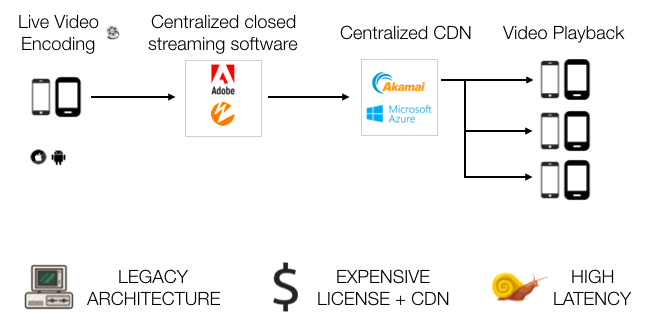
\includegraphics[width=0.95\textwidth]{static/problem-architecture-trans}
 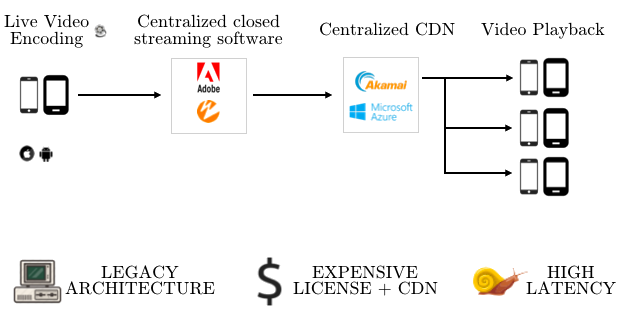
\includegraphics[width=0.95\textwidth]{static/problem-architecture-trans-cmrfont}

\end{frame}
%--- Next Frame ---%
\begin{frame}[t]\frametitle{Solution: IPCN™\textsuperscript{TM} InterPlanetary Compute Network}
% 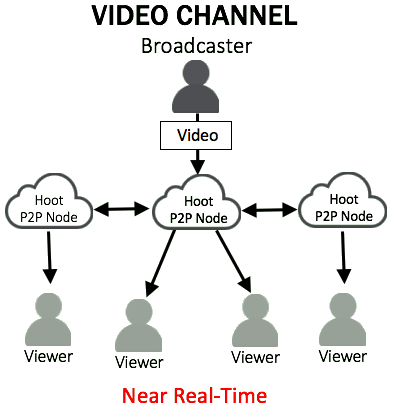
\includegraphics[scale=0.5]{static/hoot-video-architecture-channel-trans}
 % \includegraphics[width=.95\textwidth]{static/GPUCoin-solution-trans-ai}
\includegraphics[width=.95\textwidth]{static/GPUCoin-solution-trans-ai-cmrfont}

\end{frame}
%--- Next Frame ---%
\section{IPCN™}
% : InterPlanetary Compute Network
\begin{frame}[t]{IPCN: InterPlanetary Compute Network}
	%TeraFlop/PetaFlop super-computer grade
	
\includegraphics[scale=.3]{static/ipcn-p2p}
	 Uber/Airbnb for GPU computers
 \begin{itemize}
 \item Build \textbf{TeraFlop/PetaFlop super-computers} on top of the  Hoot GPUcoin \textbf{I}nter-\textbf{P}lanetary \textbf{C}ompute \textbf{N}etwork(IPCN)
 \item architecture revolving around fault tolerant redundant P2P, Blockchain, Smart Contracts, State Channels
 \item a platform to create new compute primitives using any Turing compute programming language
 \item use container technologies such as docker \& kubernetes to efficiently distribute \& use excess unused GPU compute
 \item powered by cryptocurrency micro-payments
 \item compute results verifiable using cryptographic \& mathematical properties
 \end{itemize}
\end{frame}
\section{GPUCoin}
\begin{frame}[fragile]{ GPUCoin peer to peer GPU Ðapp Network }

GPUCoin foundation is developing \href{http://gpuco.in/}{\emph{GPUCoin Network} – an Open source software}, powering a Decentralized Network of live-streaming \& distributed \textbf{GPU} accelerated computing p2p Ðapp Nodes.
 
\pause
GPUCoin Network acts as a marketplace, its open Source software allows anyone to join the network both 
 % \begin{verbatim} % \end{verbatim}

\begin{itemize}[<+-| alert@+>]
\item as a provider – selling unused network traffic, cpu, \textbf{gpu, mining} resources
\item as a customer – buying live-streaming \& distributing \textbf{GPU} accelerated computing services from other GPUCoin IPCN™\textsuperscript{TM} network providers. 

\end{itemize}
 \pause
 \textbf{P}roof \textbf{o}f \textbf{C}ompute as IPCN verification model:
 \begin{itemize}[<+-| alert@+>]
  \item compute results verifiable using cryptographic \& mathematical properties
   \item Random verification of a random selected code fragment as validation model hidden from miners to get \textbf{P}roof \textbf{o}f \textbf{C}ompute as a better alternative to Proof of Work

\end{itemize}

\end{frame}

\input{GPUCoin-tokens-frame}

\begin{frame}[fragile]{GPUCoin Use cases}
	% \begin{itemize}%needs pause
 % \setbeamercovered{transparent}%show dimmed
 % \begin{itemize}[<+->]%uncover piecewise
 \begin{itemize}[<+-| alert@+>]%uncover w highlight 
\item {Machine learning AI \& computer vision Ðapps} 
\item {Paid content consumption}
\begin{enumerate}[<+-| alert@+>]
\item Live Sports Broadcasting
\item Education 
\item Entertainment [games], Mobile Game Live streaming, E-sports
\end{enumerate}
\item {Scalable Video Services}
\item {Censorship resistant Live video Journalism}
\item {Video Enabled Ðapps}
\item {Scalable Video Services}

\end{itemize}
\pause

\Large{
Ustream, Twitch.TV, Periscope, WebEx, Maker Studio, Akamai [20B+] - will be rebuilt on the \textbf{GPUCoin IPCN™\textsuperscript{TM} Network} for the decentralized web 3.0
}

\end{frame}
%--- Next Frame ---%
\begin{frame}[t]{GPUCoin Values}
% \newcolumntype{Y}{>{\centering\arraybackslash}X}
\centering
\begin{adjustbox}{width=1\textwidth}
\begin{tabularx} {\textwidth}{|Y|Y|Y|}
 \hline
 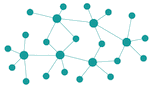
\includegraphics[scale=0.3]{./static/decentnew.png} & 
\includegraphics[scale=0.3]{./static/opensource.png} & 
\includegraphics[scale=0.3]{./static/privacy.png}\\ 
\textbf{Decentralized} & \textbf{Open source} & \textbf{Designed for privacy.png}\\
\hline
Infinitely Scalable, built using P2P architecture. Without single point of failure – no central company or server. & All source code is always visible, empowering contributions \& 100\% transparency. & Powerful encryption, Node Reputation, Layered Protection Protocols, etc.. All working to help you safely \& privately participate in the Network. \\
 \hline
\end{tabularx}
\end{adjustbox}
\end{frame}

\section{GPUCoin ICO time-line}
%--- Next Frame ---%
\begin{frame}[t]\frametitle{GPUCoin ICO Token-sale time-line}
 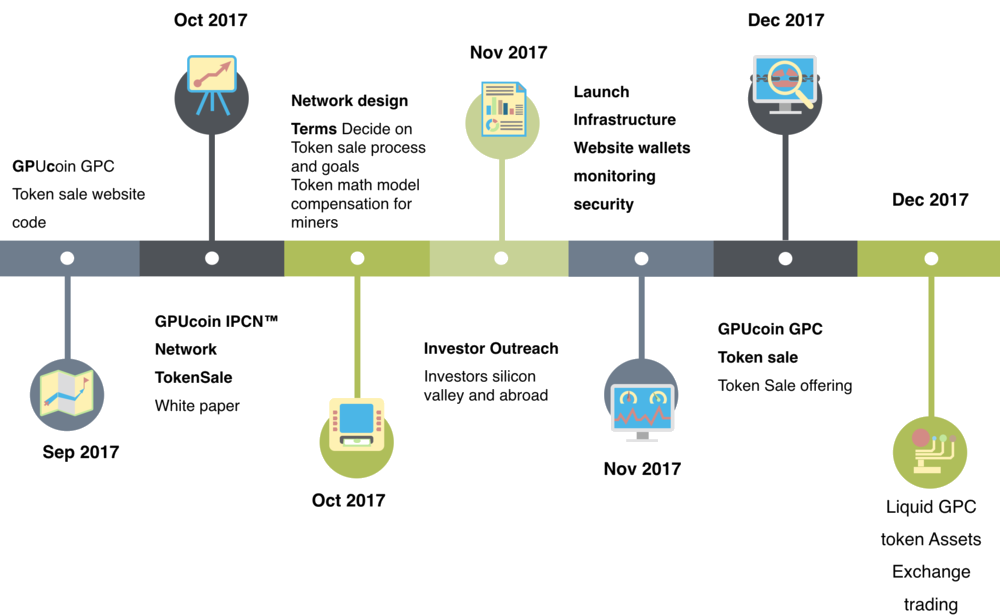
\includegraphics[width=1.0\textwidth]{static/gpc-tstimeline-trans}
\end{frame}

\begin{frame}[standout]{GPUCoin - NVIDIA/Google of crypto-currency - questions?}
\begin{center}
GPUCoin: the NVIDIA/Google of crypto-currency market 
\end{center}



\includegraphics[scale=.3]{static/ipcn-p2p}
IPCN™\textsuperscript{TM}: get the GPUCoin GPC tokens from

\includegraphics[scale=0.3]{static/hootcoin} 


 \begin{center}
\href{https://j.mp/GPUCoins}{GPUCoin™\textsuperscript{TM} ICO Tokensale}: 
\href{http://gpuco.in}{gpuco.in}
\href{mailto:founders@gpuco.in}{founders@gpuco.in} 
 % \url{https://onhoot.com/static/GPUCoin-ico}
 \end{center}
\begin{center}
% \includegraphics[scale=0.2]{static/GPUCoin-trans-256}

\textbf{GPUCoin}: the biggest \textbf{protocol} ICO since File-coin, make \textbf{mining profitable}, increase \textbf{GDP} of the crypto-currency and GPU accelerated computing markets
% to 1 Trillion \$\$
\end{center}




 \begin{center}\ccbysa\end{center}

\end{frame}


% \iffalse

% \begin{frame}[standout]
% \begin{tikzpicture}
% \node (img1) {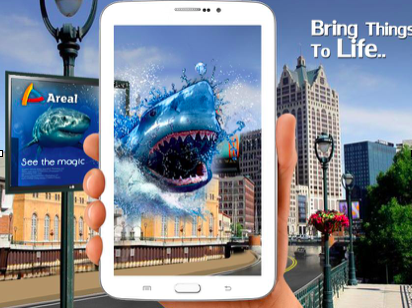
\includegraphics[height=5cm]{static/arad/arad1}};
% % \pause
% \node (img2) at (img1.south east) [xshift=-1cm] {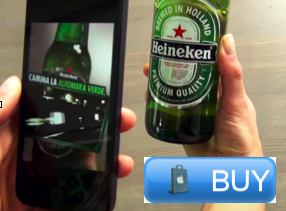
\includegraphics[height=4cm]{static/arad/arad3}};
% % \pause
% \node (img3) at (img2.south west) [xshift=-2cm,yshift=1cm] {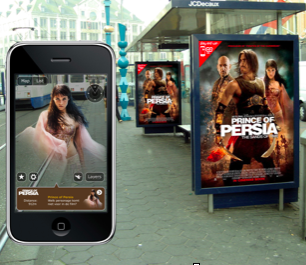
\includegraphics[height=4cm]{static/arad/arad2}};
% \pause
% \node (img4) {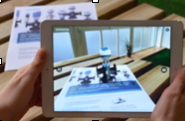
\includegraphics[height=2cm]{static/arad/arad4}};
% % \pause
% \node (img5) at (img1.south east) [yshift=-1cm] {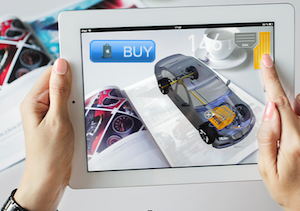
\includegraphics[height=4cm]{static/arad/arad5}};
 
% \end{tikzpicture}
 
% \end{frame}


 % \section{Description}

% \begin{frame}[allowframebreaks,fragile]{Hoot Performant AR video ads + measurable ROI = Building Adwords of video}
% \begin{footnotesize}%
% 	Video Ads have been priced historically based on CPM for impressions as it has been nearly impossible to know how much of these video ads lead to a product sale/conversion or if they even positively affect the customer ROI. Viewers do not know what action to take and how to take the said action leaving them to figure out how to follow up on the video ad they just saw, leading to a lot of drop off and lack of performance of these video ads. Hence It’s not easy  to measure effectiveness and performance of the video ads historically.

Using interactive \textbf{Hoot AR} augmented reality  ads with clear
call to actions such as a buy button or rent button below the
interactive Hoot AR ad, sales can be generated right then and there,
after the viewer interacts with the Hoot AR ad. We will be able to
charge based on sales generated from the AR interaction i.e.,
referrals and instead of pricing based on CPM or impressions we can
price based on  cost per referral(\textbf{CPR}). The CPR price becomes
the signal that drives the continuous auction engine that powers the
Hoot ad marketplace. By bringing about an innovative CPR based
business model to video ads using Augmented reality
\emph{call-to-actions} we bring the effectiveness of Google AdWords to
video ads that only used to perform as well as banner ads
before. Hence Hoot AR ads, improves the effectiveness of plain video
ads, leading to a quantum improvement in video adspend ROI much like
AdWords improved the ROI of web based banner ads, laying the
foundation for a billion dollar ads business.

% \end{footnotesize}
% \end{frame}
% \fi

\end{document}
